\documentclass{article}
\usepackage[a4paper, top=2cm, bottom=2cm, left=3cm, right=3cm]{geometry}
\usepackage{graphicx} % Required for inserting images
\usepackage{algorithm}
\usepackage{algorithmic}
\usepackage{amsmath}
\usepackage{multirow}

\title{Hybrid Distributed Sort with Bitonic Interchanges}
\author{Georgios Rousomanis (10703)\\
Department of Electrical and Computer Engineering \\
Aristotle University of Thessaloniki \\
\texttt{rousoman@ece.auth.gr}}
\date{July 2025}


\begin{document}

\maketitle

\section*{Introduction}

Sorting large datasets efficiently in distributed memory environments is a fundamental problem in parallel 
computing. This report presents an implementation of a distributed sorting algorithm based on the Bitonic sort 
paradigm, leveraging MPI for inter-process communication. The total input array of size $N = 2^{p+q}$ is 
partitioned across $2^p$ processes, each handling $2^q$ integers locally. The sorting proceeds through an 
initial local sort phase followed by iterative bitonic merging stages involving structured data exchanges 
between processes. Our implementation also incorporates optimizations such as non-blocking communication 
with buffer splitting and OpenMP-based parallelism within each process to accelerate local sorting. 
Performance evaluation on the Aristotelis HPC cluster examines the scalability and speedup characteristics 
across varying numbers of processes and input sizes, providing insights into the algorithm’s behavior and 
bottlenecks.


\section{Algorithm Overview}

The implemented algorithm is a hybrid distributed sorting method that combines local sorting with 
parallel Bitonic merging across multiple MPI processes. Each of the $2^p$ MPI processes receives a 
block of $2^q$ integers. The parameter $s$ controls the communication buffer size, dividing each local 
array into $2^{q-s}$ chunks for non-blocking communication during the pairwise exchange phase.

\subsection{Stages of the Algorithm}
The algorithm proceeds in three main stages:
\begin{enumerate}
    \item \textbf{Initial Alternating Sort:}  
    Each process locally sorts its data. Processes with even ranks sort in ascending order, while processes 
    with odd ranks sort in descending order, thus preparing a ``bitonic'' sequence across the distributed data.
    
    \item \textbf{Bitonic Merging with Pairwise Exchanges:}  
    The global merge is performed in $\log_2 (2^p) = p$ stages. At each stage, every process exchanges data 
    with a dynamically selected ``partner'' process, computed using bitwise XOR: $partner = rank \oplus 2^k$, 
    where $k$ depends on the step within the stage. This XOR operation flips the $k$-th bit of the rank, 
    effectively connecting processes whose ranks differ by a power of two. The process graph formed in this way 
    is a $p$-dimensional hypercube, where each edge represents communication between processes at Hamming 
    distance 1, 2, 4, etc. As the algorithm progresses, the sorting propagates along these hypercube edges, 
    gradually enforcing global order.

    \item \textbf{Elbow Sort:}  
    After each merging stage, each process performs an ``elbow sort'' to fully merge its local array into 
    a sorted sequence, starting from the smallest (or largest) element and expanding outward using a two-pointer
    merging technique.
\end{enumerate}

The algorithm records timing information for the local sort, communication phases, elbow sort, and total
execution time. Synchronization between processes is enforced via \texttt{MPI\_Barrier} calls to ensure 
correct timing measurements and data consistency.

\subsection{Pseudocode}

The following pseudocode summarizes the main steps of the distributed bitonic sort:

\begin{algorithm}[H]
\caption{Distributed Sort with Bitonic Interchanges}
\begin{algorithmic}[1]
\REQUIRE Local data array $local\_data$ of size $2^q$
\REQUIRE Number of processes $P = 2^p$, buffer size $B = 2^s$, process rank $r$
\ENSURE Globally sorted data distributed across all processes

\IF{$r \bmod 2 = 0$}
    \STATE \textsc{SortAscending}($local\_data$)
\ELSE
    \STATE \textsc{SortDescending}($local\_data$)
\ENDIF

\FOR{$stage = 1$ \TO $\log_2(P)$}
    \STATE $chunk \gets \lfloor r / (P / 2^{stage}) \rfloor$
    \STATE $ascending \gets (chunk \bmod 2 = 0)$

    \FOR{$step = stage - 1$ \TO $0$}
        \STATE $partner \gets r \oplus (1 \ll step)$

        \IF{$r \geq partner$}
            \STATE \textsc{NonBlockingCommunication}($local\_data$, $partner$, $B$)
        \ELSE
            \STATE \textsc{AsyncReceiveAndExchange}($local\_data$, $partner$, $B$, $ascending$)
        \ENDIF

        \STATE \textsc{Barrier}
    \ENDFOR

    \STATE \textsc{ElbowSort}($local\_data$, $ascending$)
    \STATE \textsc{Barrier}
\ENDFOR

\end{algorithmic}
\end{algorithm}

\subsection{Communication and Data Exchange}

The core of the distributed Bitonic Sort lies in the communication and data exchange between MPI processes 
during the merging phases. At each step within a stage, a process determines its partner via the XOR 
operation $partner = rank \oplus 2^k$. This operation reflects a structured traversal of a hypercube topology, 
where each dimension corresponds to one communication round. The result is a classification network where 
processes interact with others that differ in exactly one bit position of their binary rank. This structure 
enables a scalable and regular communication pattern.

Data is exchanged in chunks of size $2^s$, resulting in $2^{q-s}$ buffer splits per process. Non-blocking 
primitives (\texttt{MPI\_Isend}, \texttt{MPI\_Irecv}) are used to overlap communication and computation. 
The abstract functions \textsc{NonBlockingCommunication} and \textsc{AsyncReceiveAndExchange} encapsulate 
these steps, enabling higher-ranked processes to initiate sending early, while lower-ranked processes perform 
receives and apply directional merging logic.

This design ensures bandwidth-efficient data exchange while preserving the required bitonic structure for 
correct merges at each stage. Global consistency is maintained via barriers that synchronize all processes 
before moving to the next stage of the algorithm.

\section{Validation of the Sorting Algorithm}

To ensure correctness of the distributed bitonic sort implementation, a validation function 
is executed after the sorting completes. The validation performs two key checks:

\begin{enumerate}
    \item \textbf{Local Sorted Order:} Each process verifies that its local data chunk is sorted 
    in non-decreasing order. This is done by asserting that every element is less than or equal to 
    its successor within the local array.
    
    \item \textbf{Global Sorted Order at Process Boundaries:} Since the global sorted order spans 
    all processes, the algorithm must confirm the order between adjacent processes. Each process, 
    except the last, sends its last (maximum) element asynchronously to the next higher-ranked process. 
    Each process, except the first, receives the last element from the preceding process and asserts 
    that this received value is less than or equal to its own first (minimum) element.
\end{enumerate}

This two-level validation ensures that the data is correctly sorted both locally within each process 
and globally across the distributed dataset. Any violation triggers an assertion failure, signaling 
an error in the sorting or communication phases.

\section{Performance Overview}

This section provides an overview of the performance characteristics of the distributed bitonic sort algorithm,
focusing on how it scales with the number of processes and the size of the input array. We examine both the 
speedup achieved through parallelization and the scalability of total execution time across different 
configurations.

\subsection{Speedup by Number of Processes}

Table~\ref{tab:speedup_by_procs} illustrates the speedup achieved by increasing the number of processes for 
various total array sizes, where the size is given by $2^{p + q}$. Each row corresponds to a fixed array size, 
and each column indicates the number of processes used ($2^p$). The first valid value of each row (always $1.00$)
represents the baseline execution time. The subsequent values in the row show the speedup achieved by distributing
the workload across $2^p$ processes.

Across all array sizes, a consistent pattern emerges: the first duplication of the number of processes typically
results in a near $2\times$ speedup, indicating efficient initial parallelization. However, as the number of 
processes increases further, the incremental speedup diminishes. This is attributed to communication overheads 
and synchronization delays introduced during pairwise exchanges and elbow sorting steps of the bitonic sort 
algorithm.

\begin{table}[h]
\centering
\begin{tabular}{|c|c|c|c|c|c|c|c|c|c|}
\hline
\textbf{$p + q$} & \textbf{$p=0$} & \textbf{$p=1$} & \textbf{$p=2$} & \textbf{$p=3$} & 
\textbf{$p=4$} & \textbf{$p=5$} & \textbf{$p=6$} & \textbf{$p=7$} \\
\hline
20 & 1.00 & -    & -    & -    & -    & -    & -    & -    \\
21 & 1.00 & 1.64 & -    & -    & -    & -    & -    & -    \\
22 & 1.00 & 1.89 & 3.16 & -    & -    & -    & -    & -    \\
23 & 1.00 & 1.80 & 3.29 & 5.59 & -    & -    & -    & -    \\
24 & 1.00 & 1.98 & 3.60 & 6.17 & 10.28 & -   & -    & -    \\
25 & 1.00 & 1.92 & 3.26 & 5.90 & 10.22 & 16.60 & - & -    \\
26 & 1.00 & 1.97 & 3.53 & 6.28 & 10.26 & 17.49 & 29.26 & - \\
27 & 1.00 & 1.81 & 3.37 & 5.94 & 10.44 & 17.14 & 29.87 & 44.78 \\
28 & -    & 1.00 & 1.84 & 3.20 & 5.54  & 9.84  & 16.27 & 24.72 \\
29 & -    & -    & 1.00 & 1.79 & 3.09  & 5.47  & 9.15  & 13.97 \\
30 & -    & -    & -    & 1.00 & 1.76  & 2.92  & 5.05  & 7.95  \\
31 & -    & -    & -    & -    & 1.00  & 1.72  & 2.91  & 4.57  \\
32 & -    & -    & -    & -    & -     & 1.00  & 1.71  & 2.68  \\
33 & -    & -    & -    & -    & -     & -     & 1.00  & 1.58  \\
34 & -    & -    & -    & -    & -     & -     & -     & 1.00  \\
\hline
\end{tabular}
\caption{Speedup achieved by increasing the number of processes for various total array sizes ($2^{p+q}$).}
\label{tab:speedup_by_procs}
\end{table}

\subsection{Scalability with Global Array Size}

Figure~\ref{fig:total_time_vs_procs_by_q} shows how the total execution time scales with the total number of 
elements $2^{p+q}$, while keeping the number of elements per process constant at $2^q$. This effectively 
evaluates strong scaling by holding the local problem size fixed and increasing the total problem size and 
number of processes proportionally.

We observe that although execution time increases as the global array grows, the rate of increase is 
significantly sublinear, indicating effective parallel scaling. This is because more processes are 
recruited to handle the growing workload, reducing the per-process computational burden. However, 
the increase in total execution time is not negligible, due to factors such as inter-process communication 
and global coordination required by the bitonic merge steps.

\begin{figure}[h]
    \centering
    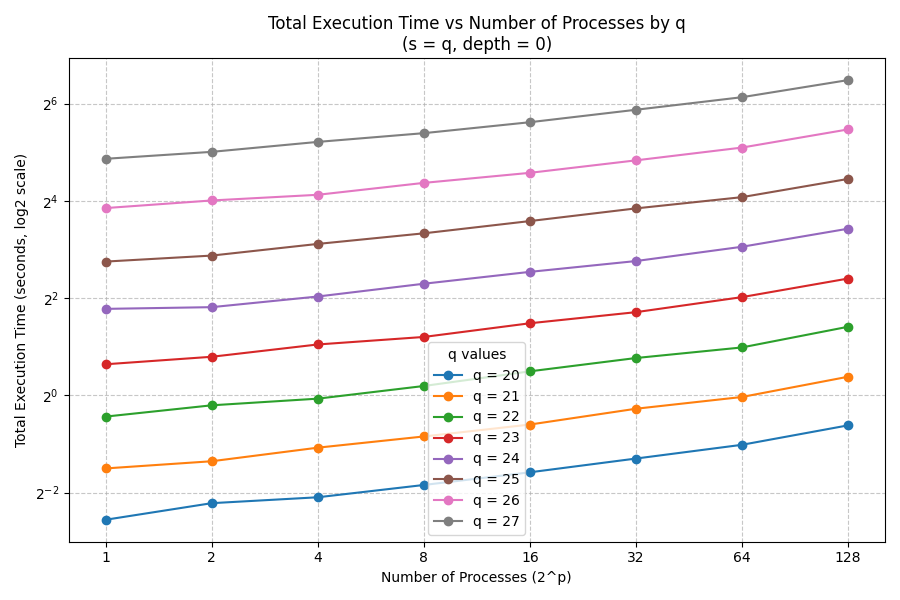
\includegraphics[width=1\linewidth]{figures/total_time_vs_procs_by_q.png}
    \caption{Total execution time vs.\ number of processes (or global size $2^{p+q}$) for fixed per-process 
    size $2^q$.}
    \label{fig:total_time_vs_procs_by_q}
\end{figure}


\section{Optimization of the Algorithm}

\subsection{Time Breakdown}

Before applying any optimizations, we analyzed how the total execution time is distributed across the 
different stages of the algorithm. Benchmarks were conducted on the Aristotelis HPC cluster using 8 
compute nodes. Figure~\ref{fig:time_breakdown} presents the execution time versus the number of processes 
$2^p$, for a fixed total input size of $2^{p+q} = 2^{27}$ integers.

We observe that for small process counts, the majority of execution time is spent on the \textit{initial sort} 
phase, which is performed locally on each process. As the number of processes increases, however, the cost of 
\textit{pairwise communication} grows significantly and eventually becomes the dominant factor, especially when 
$2^p = 128$. This trend is also reflected in Table~\ref{tab:time_breakdown}, which shows the percentage breakdown 
of time spent in each stage.

As already mentioned, doubling the number of processes from 1 to 2 results in a near-perfect speedup due to 
effective parallelization of the local sorting phase. However, further doubling leads to diminishing returns. 
This is because the computational load per process decreases, while communication overhead becomes increasingly
significant. Additionally, the complexity of synchronization and data exchange across many processes further 
hampers scalability.

\begin{figure}
    \centering
    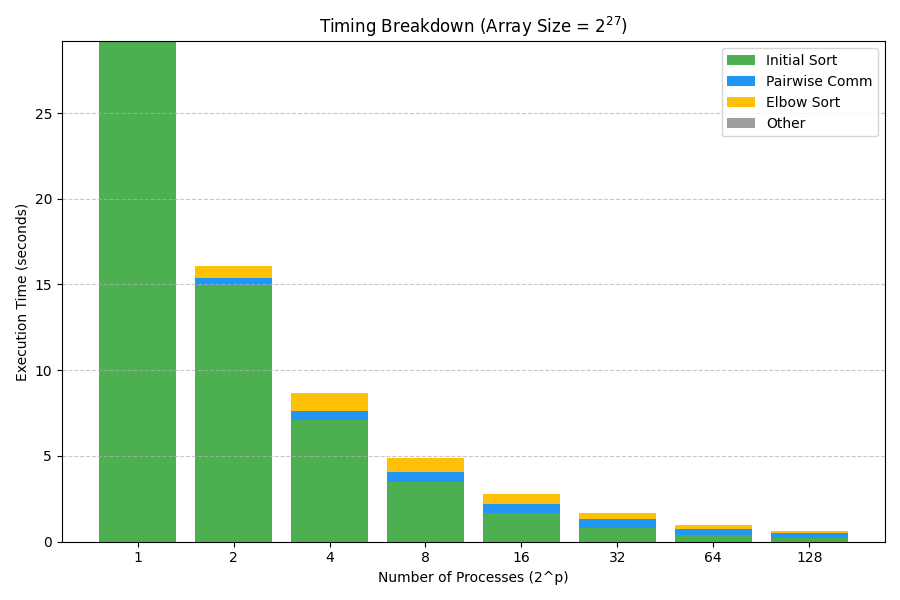
\includegraphics[width=1\linewidth]{figures/time_breakdown.png}
    \caption{Execution time breakdown per stage for total size $2^{27}$}
    \label{fig:time_breakdown}
\end{figure}

\begin{table}[h]
\centering
\begin{tabular}{|c|c|c|c|c|}
\hline
\textbf{Processes} & \textbf{Initial Sort (\%)} & \textbf{Pairwise Sort (\%)} & 
\textbf{Elbow Sort (\%)} & \textbf{Other (\%)} \\
\hline
1 & \textbf{100.00} & 0.00 & 0.00 & 0.00 \\
2 & \textbf{92.82} & 2.60 & 4.57 & 0.01 \\
4 & \textbf{81.74} & 6.50 & 11.76 & 0.01 \\
8 & \textbf{70.68} & 12.17 & 17.14 & 0.01 \\
16 & \textbf{59.46} & 19.91 & 20.62 & 0.01 \\
32 & \textbf{47.80} & 30.54 & 21.63 & 0.03 \\
64 & \textbf{39.51} & 37.67 & 22.78 & 0.04 \\
128 & 30.06 & \textbf{49.95} & 19.92 & 0.07 \\
\hline
\end{tabular}
\caption{Execution Time Breakdown (total size: $2^{p+q} = 2^{27}$)}
\label{tab:time_breakdown}
\end{table}

\subsection{Optimizing Pairwise Communication}

As illustrated in the previous subsection, \textit{pairwise communication} emerges as the primary bottleneck 
for large process counts. To address this, we experimented with splitting the communication buffer into smaller
segments. The goal of this strategy is to overlap communication with computation and enhance performance 
scalability.

Figure~\ref{fig:pairwise_comm_vs_procs} presents the pairwise communication time as a function of the number of
processes for various buffer split configurations, where the number of segments is given by $B = 2^{q-s}$. 
Splitting the communication buffer into two parts consistently improves communication performance across all 
process counts. However, further splitting into four segments does not provide additional benefit.

An interesting pattern emerges in Figure~\ref{fig:pairwise_comm_vs_procs}. The pairwise communication time 
peaks when the number of processes equals the number of compute nodes (8). This configuration forces each 
process to run on a separate node, resulting in all communication being inter-node and hence more expensive 
due to reliance on the network interface. As we increase the number of processes beyond 8, multiple processes 
begin to share the same node. This leads to more intra-node communication, which is significantly faster than 
inter-node communication, thereby reducing the total communication cost.

Table~\ref{tab:speedups_by_splits} summarizes the speedup in pairwise communication and total execution time 
when using two and four buffer splits, relative to the baseline configuration ($s = q$). The maximum speedup 
observed for communication is about 33\%, while for total execution time, it does not exceed 8\%. Additionally,
speedup diminishes as the number of processes increases. This is because the overhead from communication and 
synchronization grows, while the benefits of buffer splitting plateau.

In conclusion, while buffer splitting offers some performance improvements in specific configurations, it alone
is insufficient to achieve scalability at high process counts. These findings suggest that further optimizations
should focus on reducing the local sorting overhead, which becomes increasingly dominant as communication 
efficiency saturates.

\begin{figure}
    \centering
    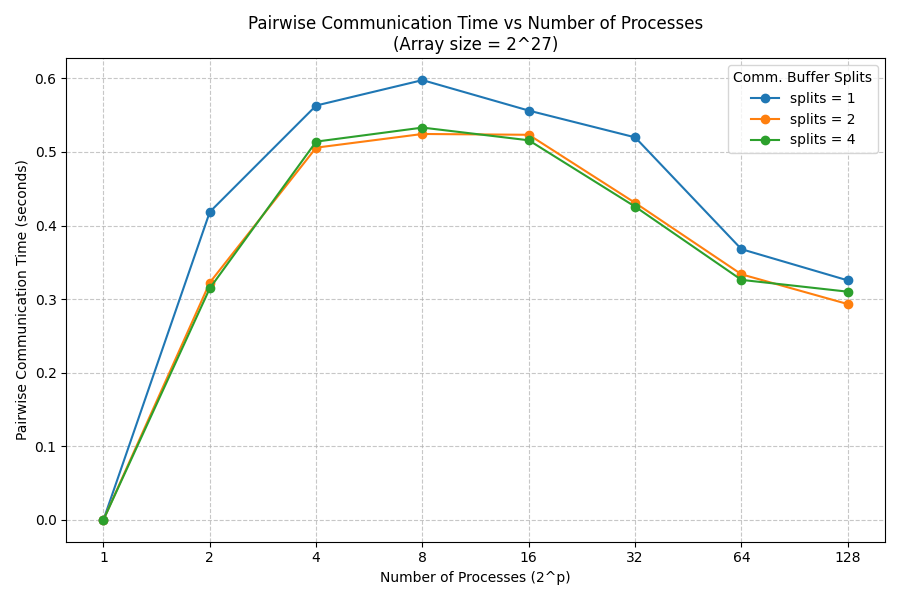
\includegraphics[width=1\linewidth]{figures/pairwise_comm_vs_procs.png}
    \caption{Pairwise communication time vs number of processes for varying communication buffer splits 
    ($B = 2^{q-s}$).}
    \label{fig:pairwise_comm_vs_procs}
\end{figure}

\begin{table}[h]
\centering
\begin{tabular}{|c|c|c|c|c|}
\hline
\multirow{2}{*}{\textbf{Processes}} & \multicolumn{2}{c|}{\textbf{Comm Speedup}} & 
\multicolumn{2}{c|}{\textbf{Total Speedup}} \\
\cline{2-5}
 & \textbf{splits: 2} & \textbf{splits: 4} & \textbf{splits: 2} & \textbf{splits: 4} \\
\hline
2   & 1.30 & 1.33 & 1.06 & 1.07 \\
4   & 1.11 & 1.10 & 1.03 & 1.01 \\
8   & 1.14 & 1.12 & 1.03 & 1.03 \\
16  & 1.06 & 1.08 & 1.04 & 1.04 \\
32  & 1.21 & 1.22 & 1.08 & 1.07 \\
64  & 1.10 & 1.13 & 1.04 & 1.04 \\
128 & 1.11 & 1.05 & 1.05 & 1.02 \\
\hline
\end{tabular}
\caption{Speedup of communication and total execution time for different split counts relative to the baseline 
($s = q$)}
\label{tab:speedups_by_splits}
\end{table}

\subsection{Optimizing Local Sorting}

As previously discussed, local sorting constitutes the primary performance bottleneck, particularly when the 
number of processes is small. To mitigate this overhead, we implemented a parallel local sorting routine using 
OpenMP. This optimization aims to exploit multicore parallelism within each process, significantly accelerating 
the initial sorting phase while keeping the implementation relatively simple and portable.

The implemented approach is based on a parallel merge sort algorithm. It recursively splits the array into 
subarrays and sorts them concurrently using OpenMP threads. Once the subarray size is small enough or the 
recursion depth becomes too large, the algorithm falls back to a serial sort. This hybrid strategy balances 
parallel performance with overhead control, ensuring efficiency across a wide range of input sizes and system 
architectures. The implementation also supports both ascending and descending ordering to remain compatible 
with the alternating sorting stages required by bitonic sort.

Table~\ref{tab:omp_speedup} and Figure~\ref{fig:total_time_vs_procs_by_depth} present the performance benefits 
of applying OpenMP-based parallelism to the local sorting phase in our distributed bitonic sort implementation. 
The benchmarks were conducted using a total problem size of $2^{27}$ elements, varying the number of processes 
as $2^p$. We evaluated two levels of parallel recursion depth (1 and 2) in the OpenMP merge sort and measured 
speedup separately for the local sorting time and the overall execution time.

As the number of processes increases, the size of the local data per process decreases, which reduces the 
effectiveness of thread-level parallelism. Nevertheless, for smaller process counts (larger per-process workload),
we observe significant speedups in both local sorting and total execution time. The gains are more pronounced in 
the initial sorting phase, as the impact of communication overhead becomes more dominant at higher process counts.
These observations demonstrate the effectiveness of hybrid parallelism, especially in scenarios where local 
computation remains a substantial portion of the overall workload.

\begin{table}[h]
\centering
\begin{tabular}{|c|c|c|c|c|}
\hline
\multirow{2}{*}{\textbf{Processes}} & \multicolumn{2}{c|}{\textbf{Speedup (Depth 1)}} & 
\multicolumn{2}{c|}{\textbf{Speedup (Depth 2)}} \\
\cline{2-5}
 & \textbf{Initial Sort} & \textbf{Total} & \textbf{Initial Sort} & \textbf{Total} \\
\hline
1 & 1.83 & 1.83 & 1.84 & 1.84 \\
2 & 1.92 & 1.82 & 1.93 & 1.83 \\
4 & 1.92 & 1.65 & 1.79 & 1.55 \\
8 & 1.88 & 1.51 & 1.86 & 1.51 \\
16 & 1.82 & 1.37 & 1.84 & 1.38 \\
32 & 1.80 & 1.31 & 1.79 & 1.30 \\
64 & 1.77 & 1.21 & 1.72 & 1.20 \\
128 & 1.66 & 1.14 & 1.59 & 1.12 \\
\hline
\end{tabular}
\caption{Speedup from OpenMP parallelism in local sorting for total problem size $2^{27}$ and varying 
number of processes.}
\label{tab:omp_speedup}
\end{table}

\begin{figure}[h]
    \centering
    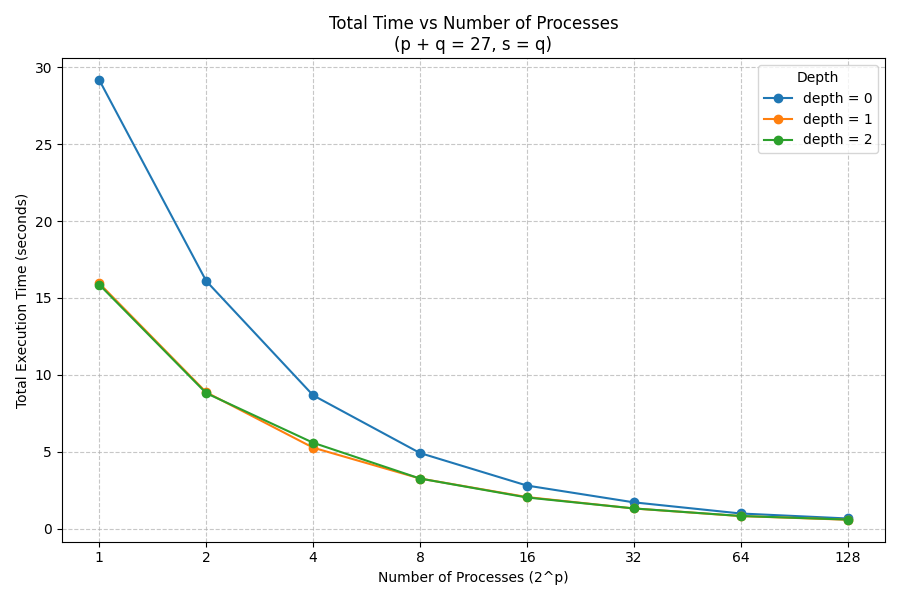
\includegraphics[width=1\linewidth]{figures/total_time_vs_procs_by_depth.png}
    \caption{Total execution time versus number of processes ($2^p$) for different OpenMP recursion depths, 
    for total input size $2^{27}$.}
    \label{fig:total_time_vs_procs_by_depth}
\end{figure}


\section*{Conclusions \& Future Work}

This work demonstrates that a hybrid distributed Bitonic sort can effectively leverage both inter-node 
parallelism through MPI and intra-node parallelism via OpenMP to improve sorting performance for large datasets. 
While initial local sorting dominates execution time for small process counts, communication overhead becomes the 
primary bottleneck as the number of processes increases. Techniques such as buffer splitting yield modest 
improvements in communication efficiency, but the scalability remains limited by inter-process data exchanges. 
Incorporating OpenMP parallelism in local sorting provides significant speedups, particularly when each process 
has a substantial workload. For future work, exploring GPU acceleration with CUDA for the initial local sorting 
phase promises further performance gains by exploiting massively parallel architectures within each compute node, 
potentially alleviating the local sorting bottleneck and improving overall scalability.


\section*{Acknowledgments}

The experiments presented in this work were conducted using the Aristotelis HPC cluster at Aristotle 
University of Thessaloniki (AUTH). We gratefully acknowledge the computational resources and support 
provided by AUTH.


\end{document}
